\documentclass{article}

\usepackage{url}
\usepackage{hyperref}
\usepackage{natbib}
%\usepackage{graphicx}
\usepackage{changepage}
\usepackage{amsmath}
\usepackage[pdftex]{graphicx}
\def\mtt{\mathtt}
\def\mrm{\mathrm}
\usepackage[margin=1.4cm]{caption}
%\usepackage{aas_macros}
%\usepackage{multirow}

\def\mnras{MNRAS}

\begin{document}
\section{The MultiNest Algorithm}
The MultiNest algorithm is a Bayesian inference tool for parameter space exploration and model selection that has come to widespread use in Astrophysics and Cosmology over the past years. 

It builds upon the nested sampling technique producing the Bayesian evidence by integrating the likelihood associated with a given set of parameters over the multidimensional parameter space, and creates samples of the posterior distribution as a by-product.

The novel way in which MultiNest represents the sampled volume by an optimized set of ellipsoids makes it especially powerful for exploring multi-modal posteriors or posteriors with curving degeneracies in high dimensions.

Our implementation follows the full description of the algorithm in \cite{2009MNRAS.398.1601F}.
\section{Performance}

\subsection{Locate the lighthouse}

While implementing our project, we used a simple (unimodal) problem from the literature to create a working infrastructure for all neccessary user and data interactions before integrating the algorithmical modules of MultiNest.  The following problem, which uses a likelihood function derived from observed data, was taken from \cite{Siv2006}:

\vspace{0.2cm}

\begin{adjustwidth*}{1.2cm}{2.cm}
A lighthouse is somewhere off a piece of straight coastline at position $\alpha$ along the shore and a distance $\beta$ out to sea. It emits a series of highly collimated flashes at random intervals and hence random azimuths. These pulses are intercepted on the coast by photo-detectors that record only the fact that a flash has occurred, but not the angle from which it came. $N$ flashes have so far been recorded at positions \{$x_k$\}. Where is the lighthouses?
 \end{adjustwidth*}
 
 \vspace{0.2cm}
 
\noindent We are told $-2 < \alpha < 2$ and $0 < \beta < 2$, so we assume uniform priors for $\alpha$ and $\beta$ in these ranges. For a given flash measurement $x_k$, it can be shown that 

\begin{equation*}
\mrm{prob}(x_k | \alpha, \beta) = \frac{\beta}{\beta^2 + (x_k - \alpha)^2},
\end{equation*}

\noindent which says the probability that the $k^\mrm{th}$ flash will be measured at $x_k$, given the lighthouse is located at ($\alpha$, $\beta$), follows the Cauchy distribution. Thus, the likelihood function is given by

\begin{equation*}
\mathcal{L}(\alpha, \beta) = \prod_{k=1}^N \mrm{prob}(x_k | \alpha, \beta).
\end{equation*}

\noindent Simulated data of $N=64$ pulses are stored in {\tt lighthouse.dat} in the {\tt DataFiles} directory. With our program, we find $\alpha = 1.24 \pm 0.19$, $\beta = 0.97 \pm 0.16$, and $\log(\mathcal{Z}) =  -161.49 \pm 0.05$, which is consistent with \cite{Siv2006}. Figure~\ref{lighthouse} shows the joint posterior distribution for $\alpha$ and $\beta$. 

\begin{figure}[h]
\begin{center}
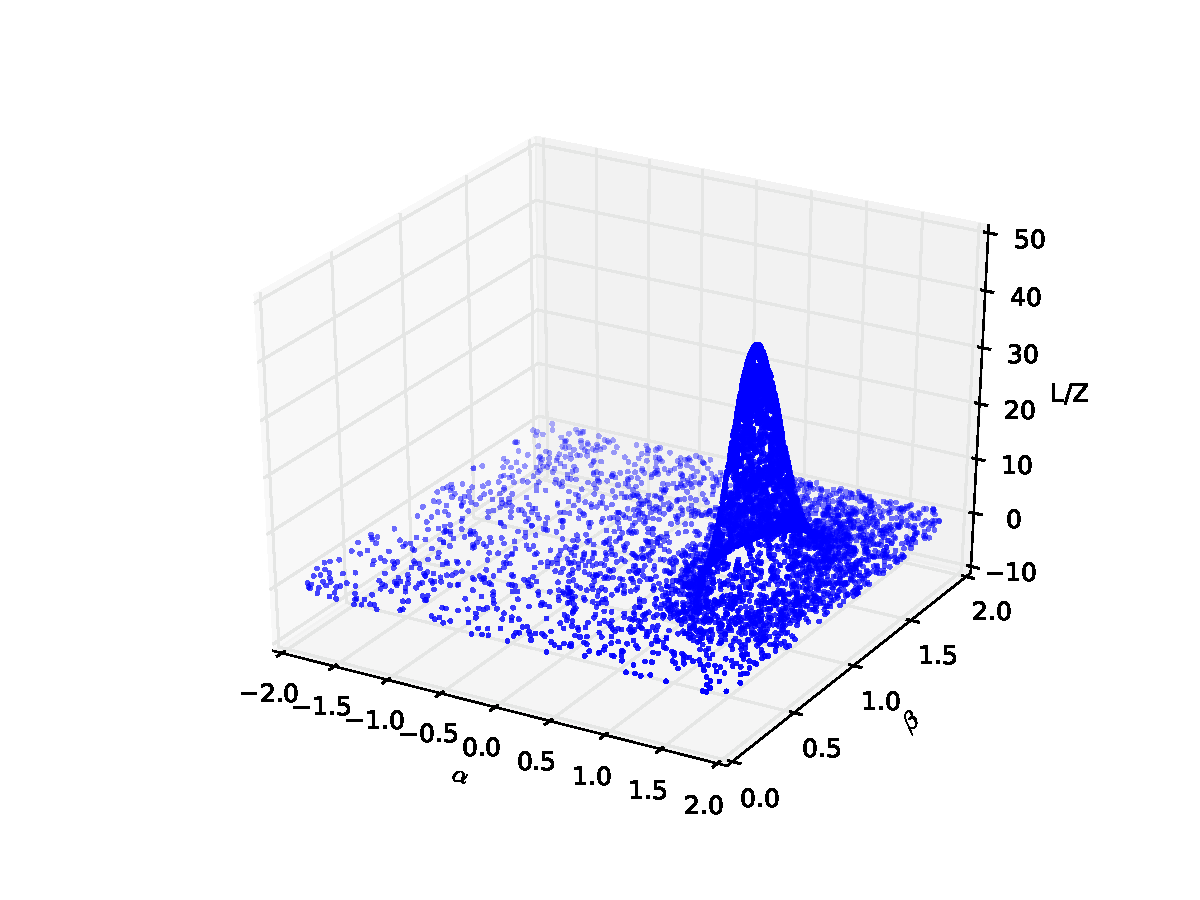
\includegraphics[width=12.0cm,trim=0cm 0cm 0cm 0cm,clip=true]{lighthouse}
\caption{Posterior probability distribution of the lighthouse location. We used 1000 active points.}
\label{lighthouse}
\end{center}
\end{figure}

\subsection{Toy model 1: ``egg-box''}
Although our MultiNest implementation is currently lacking one major feature from  \cite{2009MNRAS.398.1601F}, mode identification (described in section 5.6), we can use the test cases presented there to test our code's performance.

The first toy model is called the egg-box likelihood. It is designed to show MultiNest's performance in highly multimodal problems. Instead of deriving the likelihood function from observed data and a realistic model, it is given analytically:
\[L(\theta_1,\theta_2) = \mathrm{exp}
\left[\left\{2+\cos\left(\frac{\theta_1}{2}\right)+\cos\left(\frac{\theta_2}{2}\right)\right\}^5\right]\]
The likelihood function and its sampling returned by a run of our code with 2000 points is shown in Figure~\ref{eggbox}.

\begin{figure}
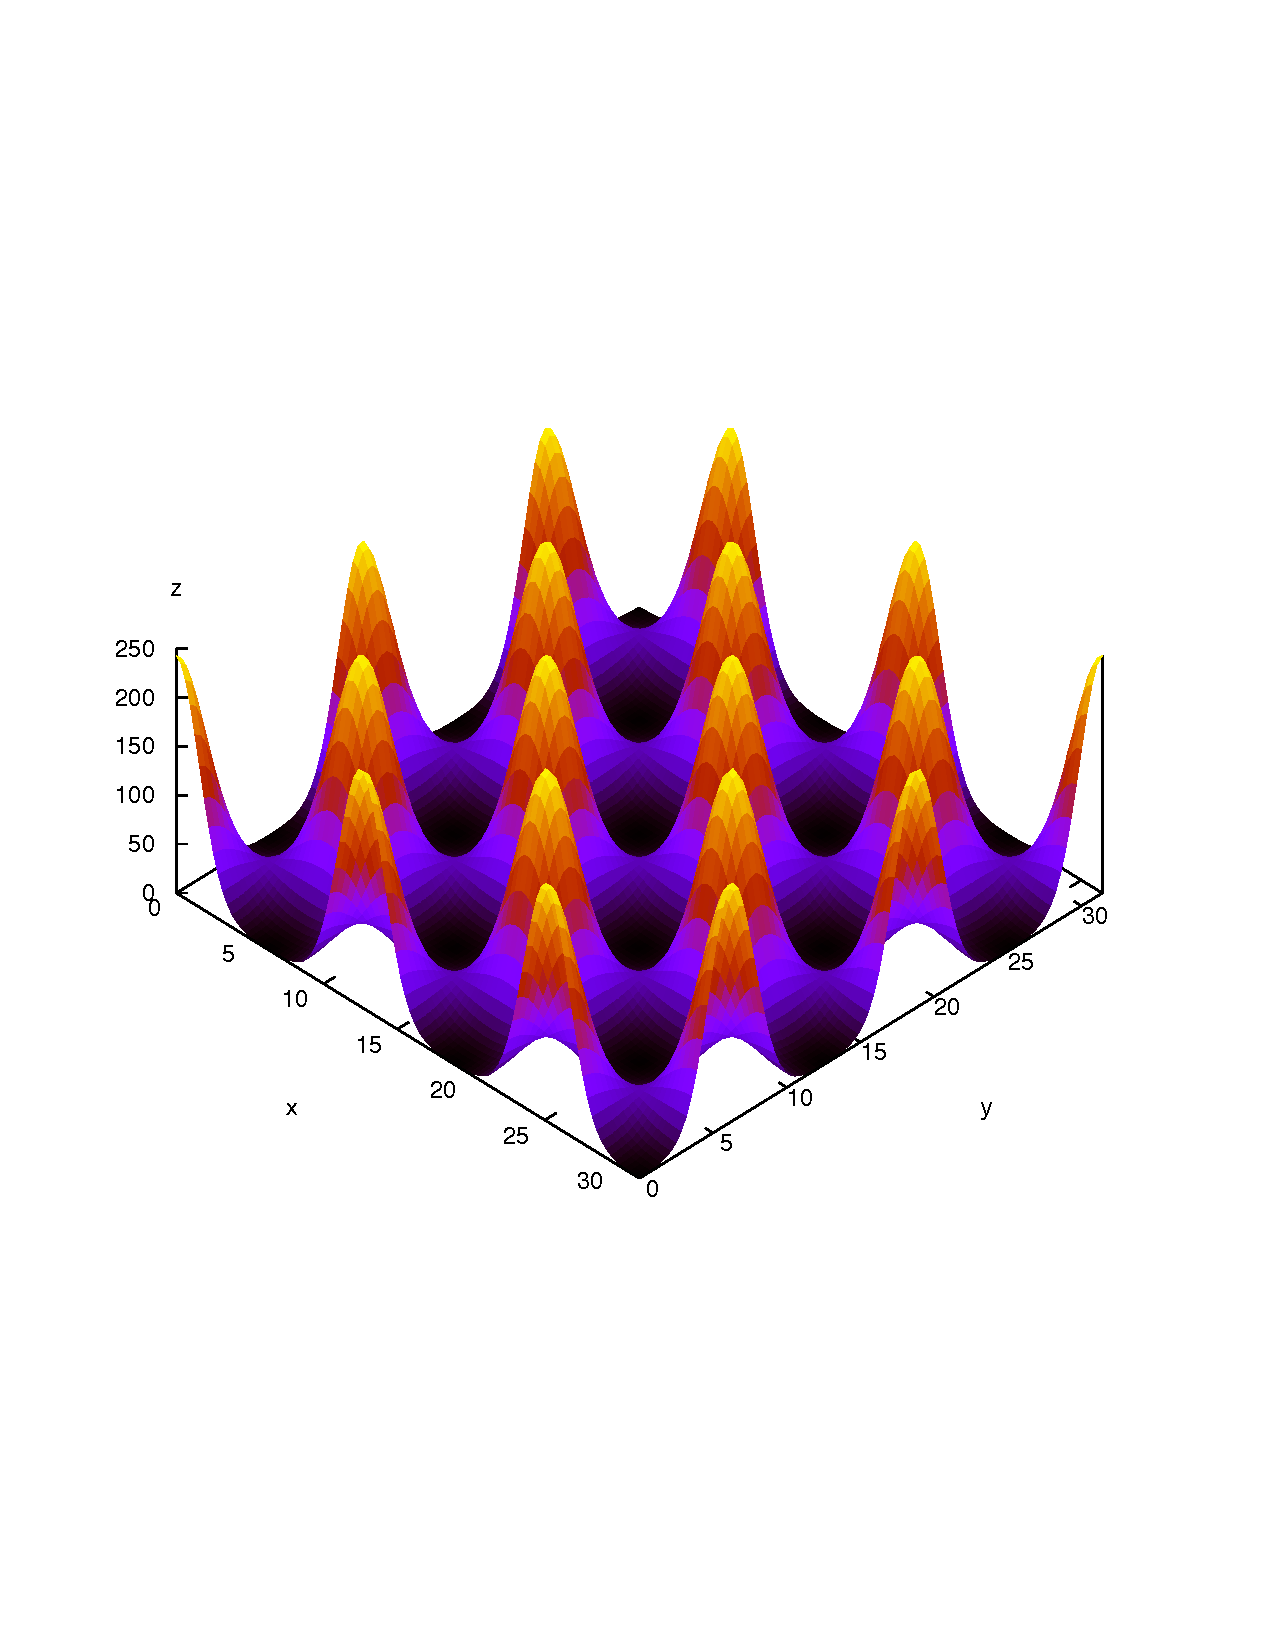
\includegraphics[width=0.5\textwidth]{eggbox_analytic.pdf}
\includegraphics[width=0.5\textwidth]{eggbox.pdf}
\caption{Analytical and sampled likelihood function of the egg-box toy model}
\label{eggbox}
\end{figure}

Given the analytical likelihood, the total log-evidence can be numerically integrated to 235.88. Our algorithm gives a result of $235.57\pm 0.06$ which is too low. Presumably, a bug either in the uniform sampling or in the final integration after convergenge limits our accuracy. This deviation will be investigated further.

\subsection{Toy model 2: ``gaussian shells''}
The second toy model in \cite{2009MNRAS.398.1601F} tests MultiNest's performance with curving degeneracies and high dimensionalities. The analytic likelihood function is given by
\[L(\theta) = \mathrm{circ}(\theta;c_1,r_1,w_1)+\mathrm{circ}(\theta;c_2,r_2,w_2)\]
where
\[ \mathrm{circ}(\theta;c,r,w) = \frac{1}{\sqrt{2\pi w^2}}\mathrm{exp}\left[-\frac{(|\theta - c|-r)^2}{2w^2}\right]\]
The two dimensional appearance of this likelihood function is shown in Figure~\ref{gaussshell}.

\begin{figure}[h]
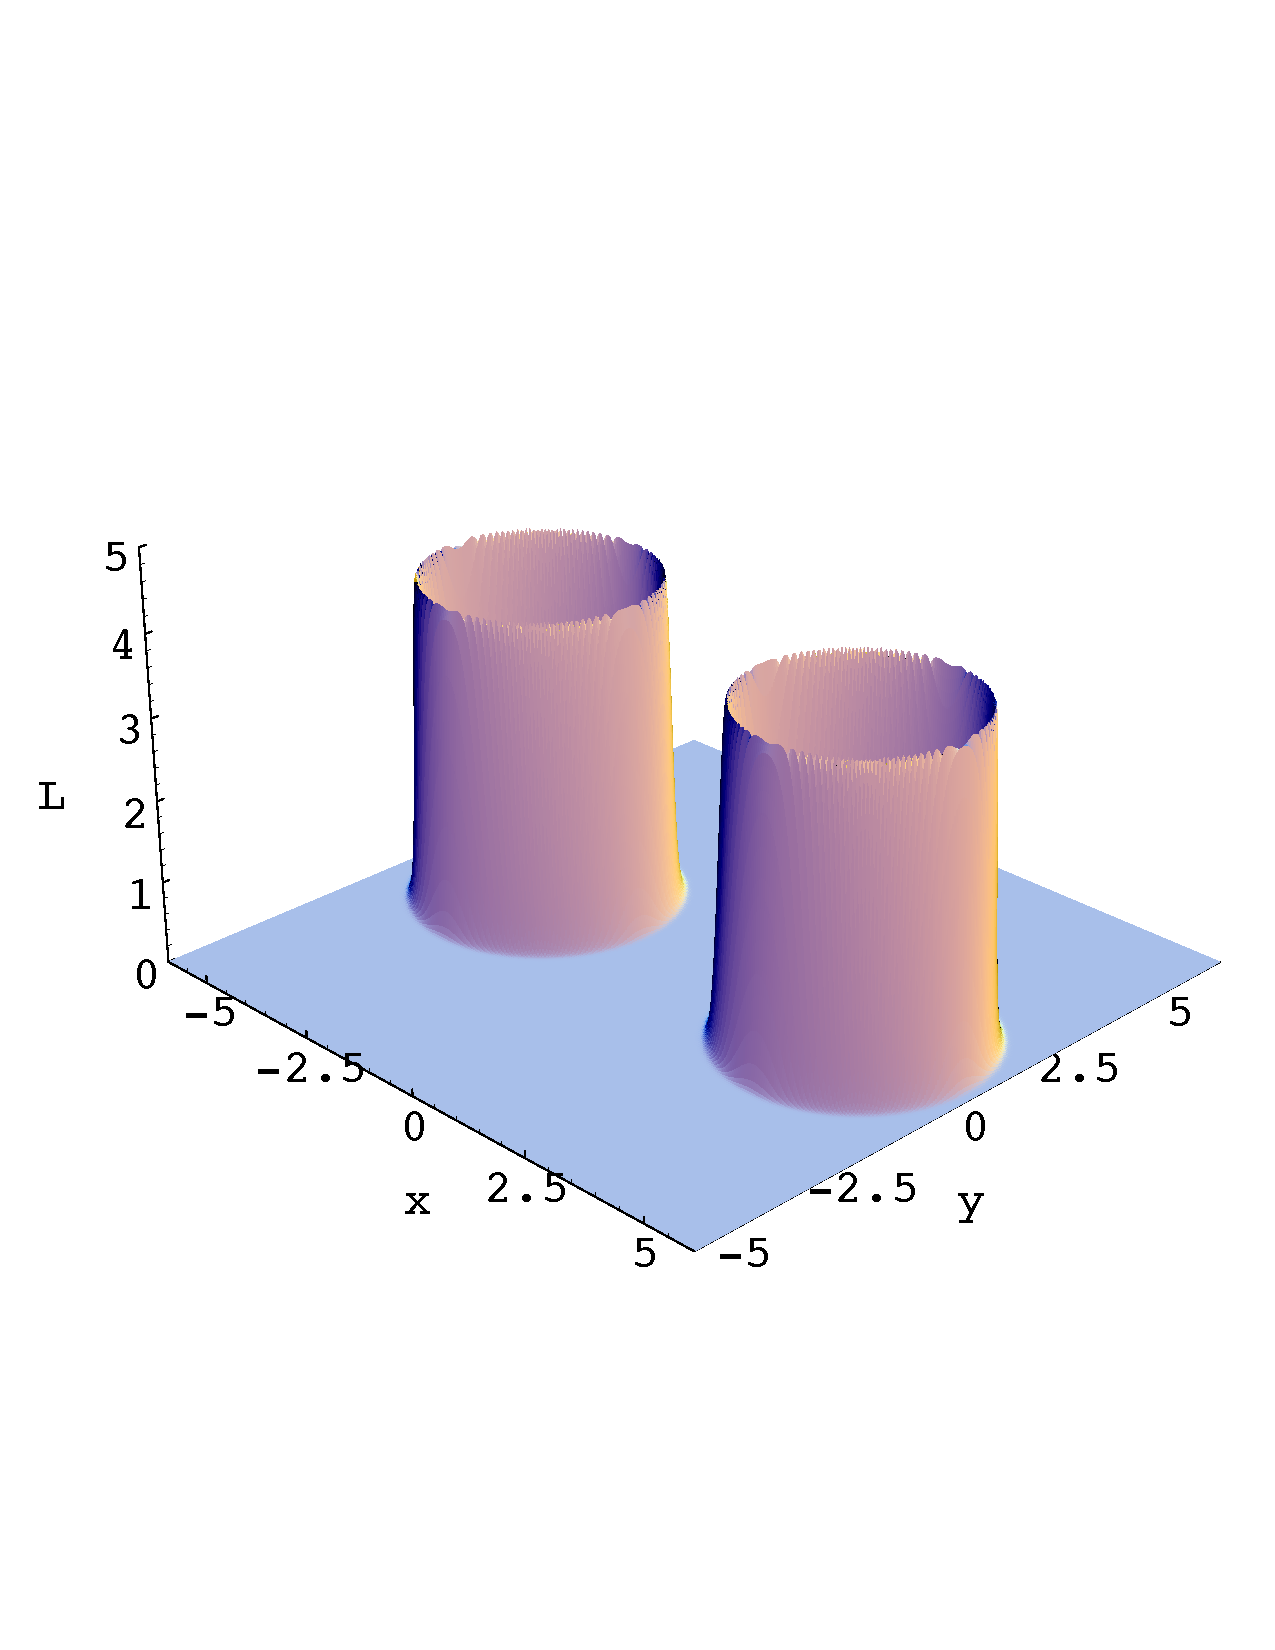
\includegraphics[width=0.5\textwidth]{gauss_shells_analytic.pdf}
\includegraphics[width=0.5\textwidth]{gauss_shells.pdf}
\caption{Analytical and sampled likelihood function of the gaussian-shells toy model}
\label{gaussshell}
\end{figure}

The total log-likelihood evaluates to $-1.75$, while our algorithm returns $-1.41\pm 0.03$  with 2000 points, which is again too low.

\subsection{Increasing Dimensionality and Sampling Efficiency}
The gaussian shell-problem can be easily expanded to arbitrary dimensions, and used to show the scaling behaviour of the number of likelihood evaluation MultiNest needs to reach a given accuracy and the sampling efficiency (successfully finding a point of higher likelihood value than the current lowest from the set of ellipsoids) it achieves.
\begin{table}\label{tab:NlikeEff}
\centering
\begin{tabular}{rrrrr}
\hline
&\multicolumn{2}{c}{\cite{2009MNRAS.398.1601F}} &\multicolumn{2}{c}{Own Implementation} \\
D&$N_{like}$ & Efficiency & $N_{like}$ & Efficiency \\ \hline
 2 &  7370 & 0.7077 & 75980 & 0.3422 \\
 5 & 17967 & 0.5102 &  ---  &  ---   \\
10 & 52901 & 0.3428 &  ---  &  ---   \\ \hline
\end{tabular}
\caption{Comparison between published and own performance of number of likelihood evaluations and sampling efficiency in gaussian-shell-problems of varying dimensionality}
\end{table}

Our algorithm at this point fails to reproduce the promised performance of MultiNest. With increasing number of dimensions, our sampling efficiency drop so fast as to prevent precise calculation of the evidence altogether. But even taking into account the lower sampling efficiency at $D=2$, our number of likelihood evaluations in unreasonably high.

Some uncertainty remains as many parameters such as the number of active points and desired final accuracy are not mentioned along with the quoted results.

\subsection{Profiled Run}
Using gprof, the following flat profile was found for a MultiNest run of the eggbox problem with 2000 points:

\begin{verbatim}
  %   cumulative   self              self     total           
 time   seconds   seconds    calls  ms/call  ms/call  name    
 35.43      6.23     6.23   388786     0.02     0.02  KMeans
 19.48      9.66     3.43  1481594     0.00     0.00  FindEnclosingEllipsoid
 16.15     12.50     2.84 218581886     0.00     0.00  Ellipsoid::mdist
 12.17     14.64     2.14     3128     0.68     5.10  Samplers::EllipsoidalPartitioning
  6.31     15.75     1.11  1870380     0.00     0.00  SelectFromGrouping
  3.24     16.32     0.57   238084     0.00     0.00  Samplers::get_newcoor
  2.96     16.84     0.52 34052242     0.00     0.00  Ellipsoid::IsMember
  1.31     17.07     0.23                             main
  0.80     17.21     0.14  1677551     0.00     0.00  Ellipsoid::Ellipsoid
  0.23     17.25     0.04 36676332     0.00     0.00  Ellipsoid::getVol
  0.11     17.31     0.02   377845     0.00     0.00  unisphere
  0.06     17.33     0.01   377845     0.00     0.00  u_in_hypercube
  0.06     17.34     0.01   377845     0.00     0.00  Ellipsoid::SampleEllipsoid
  0.06     17.35     0.01   240084     0.00     0.00  Point::transform_prior
  0.00     17.35     0.00  1481594     0.00     0.00  Ellipsoid::~Ellipsoid
  0.00     17.35     0.00   673094     0.00     0.00  Ellipsoid::getEnlFac
  0.00     17.35     0.00   477137     0.00     0.00  Ellipsoid::setEnlFac
  0.00     17.35     0.00   240084     0.00     0.00  Data::logL
  0.00     17.35     0.00   195957     0.00     0.00  Ellipsoid::getCenter
  0.00     17.35     0.00   195957     0.00     0.00  Ellipsoid::getCovMat
  0.00     17.35     0.00     3128     0.00     0.00  Samplers::CalcVtot
  0.00     17.35     0.00     2000     0.00     0.00  Point::hypercube_prior
  0.00     17.35     0.00     2000     0.00     0.00  Point::Point
  0.00     17.35     0.00        1     0.00     0.00  Data::Data
\end{verbatim}
Interestingly, the most time-consuming function appears to be K-means, a simple algorithm used for the preliminary partitioning of the data cloud, before the splitting is optimized using a more sophisticated scheme taking into account the desired ellipsoidal form of the clusters.
\section{User Instructions}
Compile the code using {\tt make}.  This program relies on the GNU Scientific Library (GSL) to do linear algebra, so be sure  you have GSL installed and that the compiler knows where to find its source files. Before running the program, run time parameters must be set in a file in the {\tt RunTimeFiles} directory. The format of run time files must be as follows. 


\begin{align*}
&\mtt{problem/data \ file}    &:& \ \ \mtt{problem \ or \ data \ file \ name}\\
&\mtt{N_{columns}}  	     &:& \ \ \mtt{\#}\\       
&\mtt{Dimension} 	            &:& \ \ \mtt{\# }\\
&\mtt{N_{points}}                &:& \ \ \mtt{\#}\\
&\mtt{efficiency \  \ factor}   &:& \ \ \mtt{1.0 \ (default \ vaule)}\\  
&\mtt{repartition \  \ factor}  &:& \ \ \mtt{1.2 \ (default \ value)}\\
&\mtt{\theta_1}                    &:& \ \ \mtt{prior \  \ \  \theta_{1,min}  \  \ \ \theta_{1,max}}\\     
&\mtt{\theta_2}                    &:& \ \ \mtt{prior \  \  \ \theta_{2,min}  \  \ \  \theta_{2,max}}\\     
\end{align*}

\noindent Here, $\theta_i$ is the $i^\mrm{th}$ parameter, {\tt prior} is the prior probability distribution for a given parameter, and the efficiency and repartition factors are optimization settings that are related to ellipsoidal partitioning and sampling. We have supplied three run time files for the test problems described above. The lighthouse problem is the only test case that requires data for likelihood evaluations, and its data file can be found in the {\tt DataFiles} directory. The current version of the code can only run these three problems, but we plan to adapt it for much more general use. 

The program takes the name of the run time file as a command-line argument. From the {\tt GrecoRothe\_MultiNest} directory, run the three test cases using the commands below.

\begin{adjustwidth*}{3.6cm}{3.5cm}
 {\tt 
 ./multinest eggbox.txt\\
./multinest gauss\_shells.txt\\
 ./multinest lighthouse.txt\\
 }
 \end{adjustwidth*}
 
\noindent If you would like to run make quick test runs with the code, lower the number of active points ({\tt Npoints}) in the run time files. Although our code can run the egg-box and Gaussian shells problems in an arbitrary number of dimensions, we have focused on 2 dimensions (2D), which allows for easy visualization and requires practical computation times. 

If the program runs successfully, it will output {\tt posterior\_pdfs.dat}, which has columns  $\theta_1$, $\theta_2$, log($\mathcal{L}$), and $\mathcal{L/Z}$. As the name implies, this file contains the necessary data to visualize the desired 2D posterior probability distributions. In addition, the program will output text similar to the following to the command-line. 

\begin{adjustwidth*}{1.2cm}{1.2cm}
{\tt
getting runtime parameters\\
creating 2000 active points in 2 dimensions\\
running MultiNest algorithm... this may take a few minutes\\
job complete!\\
**** results ****\\
number iterations = 34001\\
number reclusters = 2534\\
information: H =  8.9353 bits\\
global evidence: logZ = 235.683 +/- 0.0556484\\
****************}
\end{adjustwidth*}

As promised, the code tells us the evidence $\mathcal{Z}$, plus some additional information about how the algorithm is progressing. 

If you would like to create any of the figures in this paper, there is a python script called {\tt run\_N\_plot.py} in the {\tt scripts} directory. You will need Matplotlib and Numpy for it to work. The script takes two command-line arguments plus one optional argument. Run the script using 

\vspace{0.2cm}

\begin{adjustwidth*}{2cm}{2cm}
{\tt ./run\_N\_plot.py runtime\_filename logL|post (0|1)}
\end{adjustwidth*}

\vspace{0.2cm}

\noindent where {\tt runtime\_filename} is the name of the run time file and {\tt logL} or {\tt post} refers to the z-axis you want to plot. The optional argument is a boolean for running the full program or just plotting (1 = run full code and plot, 0 = just plot); it is set to 1 by default. There are a few examples at the top of the script file. 

\vspace{-0.3cm}

\bibliographystyle{plainnat}
\bibliography{writeup}

\end{document}
